% 
% Modelo para Trabalhos Acadêmicos (tese de doutorado, dissertação de mestrado) utilizando a classe abntex2
%
% Modificações: 07/02/2024: Wagner O. Araujo, adequação do template para a IFG - Campus: Anápolis
% ------------------------------------------------------------------------
% ------------------------------------------------------------------------

\documentclass[
	% -- opções da classe memoir --
	12pt,				% tamanho da fonte
	%openright,			% capítulos começam em pág ímpar (insere página vazia caso preciso)
	oneside,			% para impressão no anverso. Oposto a twoside
	a4paper,			% tamanho do papel. 
	% -- opções da classe abntex2 --
	chapter=TITLE,		% títulos de capítulos convertidos em letras maiúsculas
	section=TITLE,		% títulos de seções convertidos em letras maiúsculas
	%subsection=TITLE,	% títulos de subseções convertidos em letras maiúsculas
	%subsubsection=TITLE,% títulos de subsubseções convertidos em letras maiúsculas
	% -- opções do pacote babel --
	english,			% idioma adicional para hifenização
	%french,			% idioma adicional para hifenização
	%spanish,			% idioma adicional para hifenização
	brazil				% o último idioma é o principal do documento
	]{abntex2}

\usepackage{setup/ufscthesisA4-alf}
\usepackage{multirow}
\usepackage[table,xcdraw]{xcolor}
%\usepackage[utf8]{inputenc}
%\usepackage[T1]{fontenc}
%\usepackage{lmodern}
\usepackage{microtype}
\usepackage[brazil]{babel}
\usepackage{float}
\usepackage{caption}

\usepackage{booktabs}
\usepackage{blindtext}
\usepackage{siunitx}
\usepackage{amssymb}

\ProvidesPackage{verbatim}
\usepackage{fancyvrb}

\RequirePackage[vlined,titlenumbered,algo2e,ruled,portugues]{setup/algorithm2e} 



\usepackage{times}
% ---
% Filtering and Mapping Bibliographies
% ---
% Pacotes de citações
% ---
%\usepackage{csquotes}

%\usepackage[backend = biber, style = abnt]{biblatex}
% FIXME Se desejar estilo numérico de citações,  comente a linha acima e descomente a linha a seguir.
%\usepackage[
%backend = biber, 
%style = numeric-comp,
%style=abnt-numeric,
%]{biblatex}



\usepackage[alf]{abntex2cite}%Nao serve /p biblatex

\setlength\bibitemsep{\baselineskip}
%\DeclareFieldFormat{url}{Disponível~em:\addspace\url{#1}}
%\NewBibliographyString{sineloco}
%\NewBibliographyString{sinenomine}
%\DefineBibliographyStrings{brazil}{%
%	sineloco     = {\mkbibemph{S\adddot l\adddot}},
%	sinenomine   = {\mkbibemph{s\adddot n\adddot}},
%	andothers    = {\mkbibemph{et\addabbrvspace %al\adddot}},
%	in			 = {\mkbibemph{In:}}
%}

%\addbibresource{pos/references.bib} % Seus arquivos de referências para o pacote biblatex

% ---
%\DeclareSourcemap{
%	\maps[datatype=bibtex]{
%		% remove fields that are always useless
%		\map{
%			\step[fieldset=abstract, null]
%			\step[fieldset=pagetotal, null]
%		}
		% remove URLs for types that are primarily printed
%		\map{
%			\pernottype{software}
%			\pernottype{online}
%			\pernottype{report}
%			\pernottype{techreport}
%			\pernottype{standard}
%			\pernottype{manual}
%			\pernottype{misc}
%			\step[fieldset=url, null]
%			\step[fieldset=urldate, null]
%		}
%		\map{
%			\pertype{inproceedings}
%			% remove mostly redundant conference information
%			\step[fieldset=venue, null]
%			\step[fieldset=eventdate, null]
%			\step[fieldset=eventtitle, null]
%			% do not show ISBN for proceedings
%			\step[fieldset=isbn, null]
%			% Citavi bug
%			\step[fieldset=volume, null]
%		}
%	}
%}
% ---
\floatstyle{ruled}   %%% tipos: plain, boxed, ruled
\newfloat{codigo}{tbp}{lop}%[section] %%% captions with section number
\floatname{codigo}{C\'odigo}

\def\tituloprincipal{PROJETO DE CHATBOT PARA WHATSAPP: ESTUDO DE CASO PARA AVALIAÇÃO DA EXPERIÊNCIA DO USUÁRIO}

\def\autora{WAGNER OLIVEIRA DE ARAUJO}
\def\autorb{ALUNO 2}
\def\autorc{ALUNO 3}
\def\autord{ALUNO 4}

%--------------------------------------
% Palavras chave
%----------------------------------
\def\palavrachaveum{Chatbots}
\def\palavrachavedois{IA}
\def\palavrachavetres{PLN}
\def\palavrachavequatro{EX}
\def\palavrachavecinco{AttrakDiff}


% ---
% Informações de dados para CAPA e FOLHA DE ROSTO
% ---
% FIXME Substituir 'Nome completo do autor' pelo seu nome.
\autor{\autora \\ \autorb \\ \autorc \\\autord}
% FIXME Substituir 'Título do trabalho' pelo título da trabalho.
\titulo{\tituloprincipal}
% FIXME Substituir 'Subtítulo (se houver)' pelo subtítulo da trabalho.  
% Caso não tenha substítulo, comente a linha a seguir.
%\subtitulo{Subtítulo (se houver)}
% FIXME Substituir 'XXXXXX' pelo nome do seu
% orientador.
\orientador{Prof. Arlindo Rodrigues Galvão Filho, Dr.}
% FIXME Se for orientado por uma mulher, comente a linha acima e descomente a linha a seguir.
% \orientador[Orientadora]{Nome da orientadora, Dra.}
% FIXME Substituir 'XXXXXX' pelo nome do seu
% coorientador. Caso não tenha coorientador, comente a linha a seguir.
%\coorientador{Prof. XXXXXX, Dr.}
% FIXME Se for coorientado por uma mulher, comente a linha acima e descomente a linha a seguir.
% \coorientador[Coorientadora]{XXXXXX, Dra.}
% FIXME Substituir 'XXXXXX' pelo nome do Coordenador do 
% programa/curso.
% \coordenador{Prof. Fulano de Tal, Me.}
% FIXME Se for coordenadora mulher, comente a linha acima e descomente a linha a seguir.
\coordenador[Coordenador]{Prof. Alexandre Bellezi, Me.}
% FIXME Substituir '[ano da entrega]' pelo ano (ano) em que seu trabalho foi defendido.
\ano{2024}

% FIXME Substituir '[dia] de [mês] de [ano]' pela data em que ocorreu sua defesa.
\data{[dia] de [mês] de [ano]}
% FIXME Substituir '[Cidade da defesa]' pela cidade em que ocorreu sua defesa.
\local{Goiânia}
\instituicaosigla{IFG}
\instituicao{Universidade Federal de Goiás}
\def\campus{Campus: Samambaia}
% FIXME Substituir 'Dissertação/Tese' pelo tipo de trabalho (Tese, Dissertação). 
\tipotrabalho{Projeto de pesquisa apresentado como requisito parcial avaliativo da disciplina}
% FIXME Substituir '[licenciado/bacharel] em [nome do título obtido]' pela grau adequado.
\formacao{Programa de Linguagem Natural}
% FIXME Substituir '[licenciado/bacharel]' pelo nivel adequado.
\nivel{bacharel}
% FIXME Substituir 'Curso de Graduação em [XXXXXXXX]' pela curso adequado.
\programa{Programa de Pós-graduação em Ciência da Computação}
% FIXME Substituir 'Campus XXXXXX ou Centro de XXXXXX' pelo campus ou centro adequado.
%\centro{Campus [XXXXXX] ou Centro de [XXXXXX]}
\preambulo
{%
\imprimirtipotrabalho~\imprimirformacao~do curso~\imprimirprograma~da~\imprimircentro~\imprimirinstituicao~--~\campus.
}
% ---

% ---
% Arquivos de definição
% ---
\def\spf{Servi\c{c}o P\'ublico Federal}

\def\setor{Campus: An\'apolis}

%-----Ficha catalografica
\def\ano{2024}
\def\sigla{IFG}
\def\curso{Ciência da Computação}
\def\palavrachaveum{Erosão}
\def\palavrachavedois{Ravina}
\def\palavrachavetres{Voçoroca}
\def\palavrachavequatro{Geotecnia}
\def\palavrachavecinco{Monitoramento}
\def\nomeorient{Wagner Oliveira de}
\def\sobrenomeorient{Araujo}
\def\sigorient{orient}
\def\tcc{Trabalho de Conclusão de Curso (Graduação)}
\def\cdu{CDU 02:141:005.7}
\def\codnome{A663c}
\def\cip{Dados Internacionais de Catalogação na Publição (CIP)}
\def\bibliotecario{Matheus Rocha Piacenti}
\def\cbr{CRB1/2992}

%-----TERMO DE AUTORIZAÇÃO PARA DISPONIBILIZAÇÃO
\def\titulo{\tituloprincipal}
\def\biblioteca{SISTEMA INTEGRADO DE BIBLIOTECAS}
\def\campus{Campus: Samambaia}%Capa e mancha
\def\alunonome{Wagner Oliveira de}
\def\alunosobre{Araujo}
\def\matricula{20171060130231}
\def\diaata{8}
\def\mesata{julho}
\def\entidade{Instituto Federal de Educa\c{c}\~ao, Ci\^encia e Tecnologia de Goi\'as}
\def\todaydia{%
\ifnum \day < 10 0\fi%
\number\day
}
\def\todayano{%
\number\year}
%---------------------------------
%-----ATA DE APROVAÇÃO
\def\ministerio{MINISTÉRIO DA EDUCAÇÃO}
\def\secretaria{SECRETARIA DE EDUCAÇÃO PROFISSIONAL E TECNOLÓGICA}
\def\instituto{INSTITUTO FEDERAL DE EDUCAÇÃO, CIÊNCIA E TECNOLOGIA}
\def\reitoria{PRÓ-REITORIA DE PESQUISA E PÓS-GRADUAÇÃO}
\def\termo{\textbf{TERMO DE AUTORIZAÇÃO PARA DISPONIBILIZAÇÃO\\ NO REPOSITÓRIO DIGITAL DO IFG--ReDi IFG}}
\def\termodois{Com base do disposto na Lei Federal nº 9.610/98, AUTORIZO o~\entidade, a disponibilizar gratuitamente o documento no Repositório Digital (ReDi~\sigla), sem ressarcimento de direitos autorais, conforme permiss\~ao assinada abaixo, em formato digital para fins de leitura, download e impressão, a título de divulgação de produção técnico-científica no IFG.}
\def\declaracao{DECLARAÇÃO DE DISTRIBUIÇÃO NÃO-EXCLUSIVA}
\def\termotres{~obteve autorização de quaisquer materiais inclusos no documento do qual não detém os direitos de autor(a), para conceder ao \entidade~os direitos requeridos e que este material cujos direitos autorais são de terceiros, estão claramente identificados e reconhecidos no texto ou conteúdo do documento entregue;}

%Dados para a ATA
\def\diaata{8}
\def\mesata{julho}
\def\hinicial{14}\def\minicial{00}
\def\hfinal{15}\def\mfinal{45}
\def\notanumerico{9,2}\def\notaextenso{nove v\'irgula dois}

\def\curso{Ci\^encia da Computa\c{c}\~ao}
\def\orientadora{Angela Cust\'odia Guimar\~aes Queiroz}

\def\nomeconvum{Maria T\^amara}%Ata e outros
\def\sobrenomeconvum{de Moraes Guimar\~aes Silva}%Ata e outros

\def\membroum{\nomeconvum~\sobrenomeconvum}%Ata
\def\nomeconvdois{Camilla}%Folha de aprovação

\def\nomeconvdois{Camilla}%Folha de aprovação
\def\sobrenomeconvdois{Rodrigues Borges}%Folha de aprovação
\def\membrodois{\nomeconvdois~\sobrenomeconvdois}%Ata
\def\asseletronica{(\textbf{assinado eletronicamente})}



% ---
% Configurações de aparência do PDF final
% ---
% alterando o aspecto da cor azul
\definecolor{blue}{RGB}{41,5,195}
% informações do PDF
\makeatletter
\hypersetup{
     	%pagebackref=true,
		pdftitle={\@title}, 
		pdfauthor={\@author},
    	pdfsubject={\imprimirpreambulo},
	    pdfcreator={LaTeX with abnTeX2},
		pdfkeywords={\palavrachaveum, \palavrachavedois, \palavrachavetres,\palavrachavequatro,\palavrachavecinco}, 
		colorlinks=true,       		% false: boxed links; true: colored links
    	linkcolor=black,%blue,          	% color of internal links
    	citecolor=black,%blue,        		% color of links to bibliography
    	filecolor=black,%magenta,      		% color of file links
		urlcolor=black,%blue,
		bookmarksdepth=4
}
\makeatother
% ---

% ---
% compila a lista de abreviaturas e siglas e a lista de símbolos
% ---
% Para habilitar utilize pre \imprimirlistadesiglas
% Declaração das siglas
\siglalista{ABNT}{Associação Brasileira de Normas Técnicas}

% Declaração dos simbolos
\simbololista{C}{\ensuremath{C}}{Circunferência de um círculo}
\simbololista{pi}{\ensuremath{\pi}}{Número pi} 
\simbololista{r}{\ensuremath{r}}{Raio de um círculo}
\simbololista{A}{\ensuremath{A}}{Área de um círculo}

% compila a lista de abreviaturas e siglas e a lista de símbolos
\makenoidxglossaries 
% ---

% ---
% compila o indice
% ---
\makeindex
% ---


% ----
% Início do documento
% ----
\begin{document}

% Seleciona o idioma do documento (conforme pacotes do babel)
%\selectlanguage{english}
\selectlanguage{brazil}

% Retira espaço extra obsoleto entre as frases.
\frenchspacing 

% Espaçamento 1.5 entre linhas
\OnehalfSpacing

% Corrige justificação
%\sloppy

% ----------------------------------------------------------
% ELEMENTOS PRÉ-TEXTUAIS
% ----------------------------------------------------------
\pretextual %a macro \pretextual é acionado automaticamente no início de \begin{document}
% ---
% Capa, folha de rosto, ficha catalográfica, errata, folha de aprovação
% Dedicatória, agradecimentos, epígrafe, resumos, listas
% ---
% ---
% Capa
% ---
\imprimircapa
% ---

% ---
% Folha de rosto
% (o * indica que haverá a ficha catalográfica)
% ---
\imprimirfolhaderosto
% ---

% ---
% Ficha Catalografica em pdf e código
% 
% ---

%\begin{fichacatalografica}
%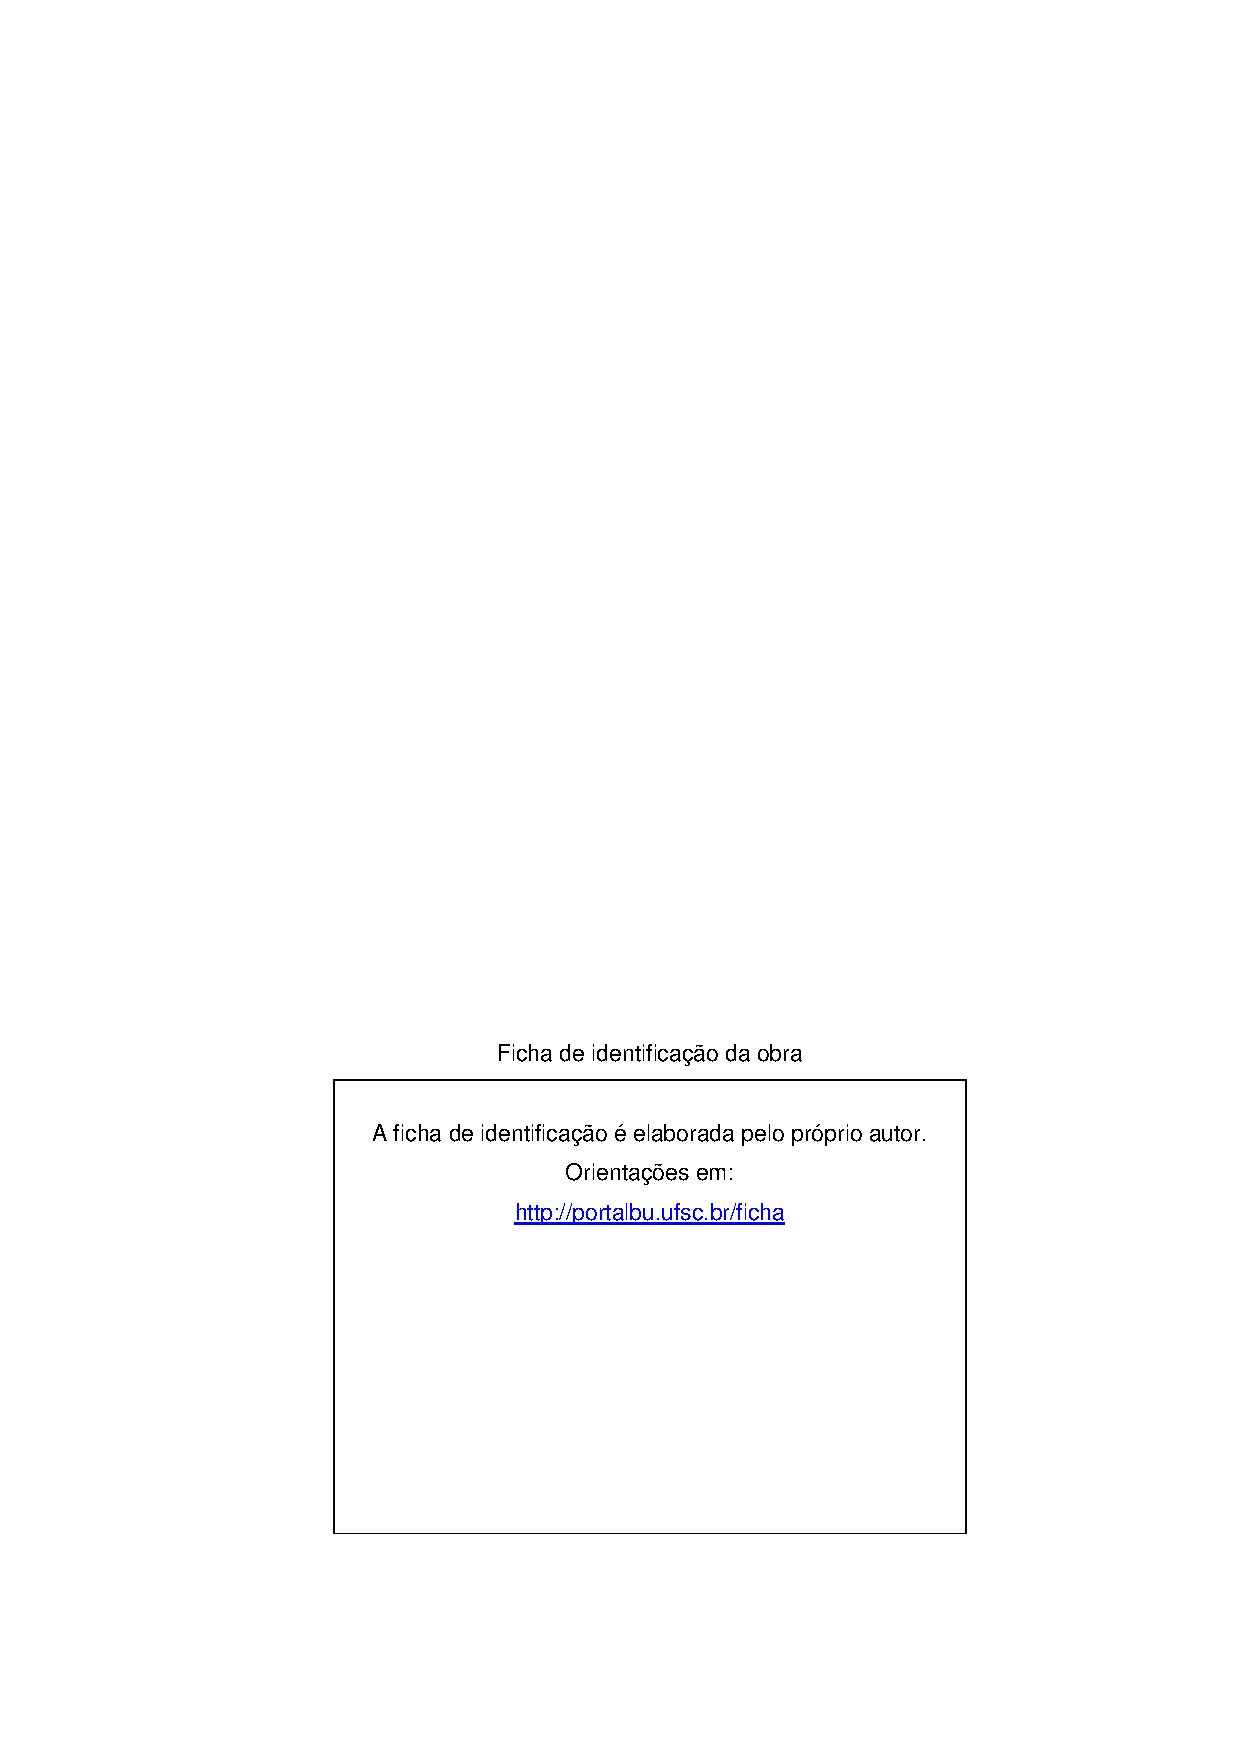
\includepdf{pre/Ficha_Catalografica.pdf}
%\end{fichacatalografica}

%\begin{fichacatalografica}
\vspace*{12cm} % Posição vertical
%\hrule % Linha horizontal

\begin{center} % Minipage Centralizado
\small{\textbf{\cip}}
\framebox[120mm]{%Inicio da caixa
\begin{minipage}{105mm} % Largura [c]{12.5cm}
\begin{flushleft}
\codnome
\end{flushleft}
\imprimirautor

\hspace{0.5cm} \imprimirtitulo / \imprimirautor. --
\imprimirlocal:~\sigla,~\ano.

\hspace{0.5cm} \pageref{LastPage} p. : il.~color.; 30 cm.\\

\hspace{0.5cm} \imprimirorientadorRotulo:~ \imprimirorientador\\

\hspace{0.5cm}
\parbox[t]{\textwidth}{\tcc~--~\imprimirinstituicao,~\campus~--~\curso~\ano.}\\

\hspace{0.5cm}
1. \palavrachaveum.
2. \palavrachavedois.
3. \palavrachavetres.
4. \palavrachavequatro.
5. \palavrachavecinco.
I. \MakeUppercase{\sobrenomeorient},~\nomeorient~\sigorient..
%II. Universidade xxx.
%III. Faculdade de xxx.
II. T\'tulo.\\

%\hspace{7.75cm} \cdu\\
\begin{flushright}
    						\cdu
\end{flushright}%
%\hspace{8.75cm}
\end{minipage}
}%Fim caixa
\par
\vspace{0.1cm}
Ficha catalogr\'afica elaborada pelo bibliotec\'ario~\bibliotecario~\cbr
\par
Biblioteca Clarice Lispector
\par
\imprimirinstituicao
\par
Campus: An\'apolis

\end{center}

%\hrule
\end{fichacatalografica}

%----------------------------------------------


% ---
% Inserir folha de aprovação
% ---
%\begin{folhadeaprovacao}
	\OnehalfSpacing
	\centering
	\imprimirautor\\%
	\vspace*{10pt}		
	\textbf{\imprimirtitulo}%
	\ifnotempty{\imprimirsubtitulo}{~\imprimirsubtitulo}\\%
	%		\vspace*{31.5pt}%3\baselineskip
	\vspace*{\baselineskip}
	%\begin{minipage}{\textwidth}
	% ~do~\imprimirprograma~do~\imprimircentro~da~\imprimirinstituicao~para~a~obtencao~do~título~de~\imprimirformacao.
	Este~\imprimirtipotrabalho~foi julgado adequado para obten\c{c}\~ao do T\'itulo de ''\imprimirformacao'' e aprovado em sua forma final pelo~\imprimirprograma. \\
		\vspace*{\baselineskip}
	\imprimirlocal, \imprimirdata. \\
	\vspace*{2\baselineskip}
	\assinatura{\OnehalfSpacing\imprimircoordenador \\ \imprimircoordenadorRotulo~do Curso}
	\vspace*{2\baselineskip}
	\textbf{Banca Examinadora:} \\
	\vspace*{\baselineskip}
	\assinatura{\OnehalfSpacing\imprimirorientador \\ \imprimirorientadorRotulo}
	%\end{minipage}%
	\vspace*{\baselineskip}
	\assinatura{Prof.(a) xxxx, Dr(a).\\
	Avaliador(a) \\
	Institui\c{c}\~ao xxxx}

	\vspace*{\baselineskip}
	\assinatura{Prof.(a) xxxx, Dr(a).\\
	Avaliador(a) \\
	Institui\c{c}\~ao xxxx}


\end{folhadeaprovacao}
% ---

% ---
% Inserir folha de ata da seção pública de tcc
% ---
%\linespread{0.87}

%--------Cabeçalho do documento
\noindent\begin{minipage}[c][1.5cm][c]{3.5cm}
%\includegraphics[height=1.5cm]{./figuras/logoEvangelica.eps}

\includegraphics[width=1.5 \textwidth]{./outros/fig/IFGAnapolisHor2.png}
\end{minipage}\quad\quad\quad\qquad
\begin{minipage}{12cm}%10cm
\scriptsize\textbf{\ministerio}\\%\sc
\textbf{\secretaria}\\
\textbf{\instituto}\\
\textbf{\reitoria}\\
\end{minipage}
\vspace{1cm}
%---------------------------------------------------------------------------------------


\begin{center}
	\textbf{ATA N\textsuperscript{o} 20/2022.1}\\
	\footnotesize{\MakeUppercase{\textbf{Ata da sess\~ao p\'ublica de apresenta\c{c}\~ao do trabalho de conclus\~ao de curso 2}}}
\end{center}
\vspace{1.0cm}
\noindent Aos~0\diaata~dias do m\^es de~\mesata~do ano de dois mil e vinte dois, \'as~\hinicial~horas, por meio de webconfer\^encia utilizando Google Meet, foi realizada a sess\~ao p\'ublica de apresenta\c{c}\~ao do Trabalho de Conclus\~ao 2 da Graduando~\textbf{\alunonome~\alunosobre}~(matr\'icula~\matricula) do curso de~\curso. A banca foi composta pelos seguintes membros:~\orientadora,~\membroum,~\membrodois, sob a presid\^encia da primeira. O trabalho de conclus\~ao de curso tem como t\'itulo ``\textbf{\titulo}'', da \'area de Geotecnia, sob orienta\c{c}\~ao da Prof\textsuperscript{a}~\orientadora. Ap\'os a apresenta\c{c}\~ao do Trabalho de Conclus\~ao de Curso 2, tendo sido o autor arguido pela Banca Examinadora, a nota obtida foi~\notanumerico~(\notaextenso).
\\
\\
\noindent Encerra-se a presente sess\~ao \'as~\hfinal~horas~e~\mfinal~minutos. Eu Prof\textsuperscript{a}.~\orientadora, dato e assino a presente ata que segue assinada por todos os membros da Banca e pelo graduando.
\vspace{1.0cm}
\small{
\begin{center}
\begin{tabular}{c}
\multicolumn{1}{c}{\asseletronica} \\ 
\multicolumn{1}{c}{Prof\textsuperscript{a}~\orientadora} \\ 
\multicolumn{1}{c}{} \\ 
\asseletronica \\ 
\multicolumn{1}{c}{Prof\textsuperscript{a}~\membroum~} \\ 
\multicolumn{1}{c}{~} \\ 
\asseletronica\\
%
\includegraphics[width=0.30 \textwidth]{./outros/fig/AssDaniel.jpg} \\ %\hrulefill comando para linha
\multicolumn{1}{c}{Prof\textsuperscript{a}~\membrodois~} \\ 
\multicolumn{1}{c}{~} \\ 
\includegraphics[width=0.25 \textwidth]{./outros/fig/minhaAssinatura.png} \\
\multicolumn{1}{c}{\textbf{\alunonome~\alunosobre}} \\
\multicolumn{1}{c}{(Graduando)} \\
\multicolumn{1}{c}{~} \\ 
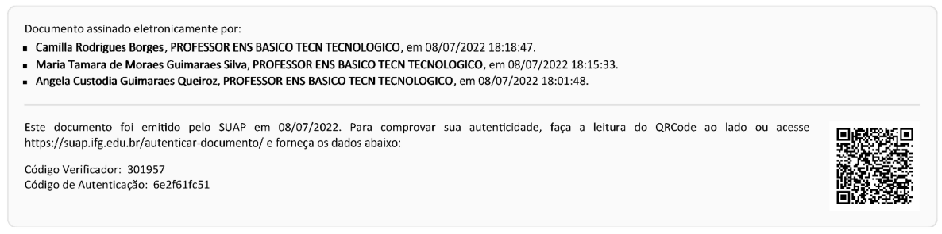
\includegraphics[width=0.97 \textwidth]{./outros/fig/QR_CODE_V2.pdf}
\\
\end{tabular}
\end{center}
}

\linespread{1.3}
\newpage





% ---
% Inserir folha de autorização para disponibilização
% ---
%\linespread{0.87}
%--------Cabeçalho do documento
\noindent\begin{minipage}[c][1.5cm][c]{3.5cm}

\includegraphics[width=1.5 \textwidth]{./outros/fig/IFGAnapolisHor2.png}
\end{minipage}\quad\quad\quad\qquad
\begin{minipage}{12cm}%10cm
\scriptsize\textbf{\ministerio}\\
\textbf{\secretaria}\\
\textbf{\instituto}\\
\textbf{\MakeTextUppercase{\campus}}\\
\textbf{\biblioteca}\\
\end{minipage}
%\vspace{-0.1cm}
\small{
\begin{center}
	\termo
\end{center}

%Com base do disposto na Lei Federal nº 9.610/98, AUTORIZO o~\entidade, a disponibilizar gratuitamente o documento no Reposit\'orio Digital (ReDi~\sigla), sem ressarcimento de direitos autorais, conforme permiss\~ao assinada abaixo, em formato digital para fins de leitura, download e impress\~ao, a t\'itulo de divulga\c{c}\~ao de produ\c{c}\~ao t\'ecnico-cient\'ifica no IFG.
\termodois

\noindent \textbf{Identifica\c{c}\~ao de Produ\c{c}\~ao T\'ecnico-Cient\'ifica}

\begin{tabular}{lllll}
\lbrack ~~\rbrack & Tese &  & \lbrack ~~\rbrack & Artigo Cient\'ifico \\ 
\lbrack ~~\rbrack & Disserta\c{c}\~ao &  & \lbrack ~~\rbrack & Cap\'itulo de Livro \\ 
\lbrack ~~\rbrack & Monografia -- Especializa\c{c}\~ao &  & \lbrack ~~\rbrack & Livro \\ 
\lbrack X\rbrack & TCC -- Gradua\c{c}\~ao &  & \lbrack ~~\rbrack & Trabalho Apresentado em Evento \\ 
\lbrack ~~\rbrack & Produto T\'ecnico e Educacional -- Tipo: & \multicolumn{3}{l}{\hrulefill} \\ 
\end{tabular}

\quad

\noindent Nome Completo do Autor:~\textbf{\alunonome~\alunosobre}

\noindent Matr\'icula:~\textbf{\matricula}

\noindent T\'ituto do Trabalho:~\textbf{\tituloprincipal}

\noindent \textbf{Autoriza\c{c}\~ao -- Marque uma das op\c{c}\~oes}

\begin{enumerate}
	\item (X) Autorizo disponibilizar meu trabalho no Reposit\'orio Digital do IFG (acesso aberto);
	\item (~) Autorizo disponibilizar meu trabalho no Reposit\'orio Digital do IFG somente ap\'os a data 20/10/20 (Embargo);
	\item (~) N\~ao autorizo disponibilizar meu trabalho no Reposit\'orio Digital do IFG (acesso restrito)
\end{enumerate}

\noindent Ao indicar a op\c{c}\~ao \textbf{2 ou 3}, marque a justificativa:
\begin{description}
	\item[(~~)] O documento est\'a sujeito a registro de patente.
	\item[(~~)] O documento pode vir a ser publicado como livro, cap\'itulo de livro ou artigo.
	\item[(~~)] Outra justificativa: \hrulefill
\end{description}

\begin{center}
	\textbf{\declaracao}
\end{center}

\noindent O(A) referido(a) autor(a) declara que:

\textbf{(i)}~o documento \'e seu trabalho original, det\'em os direitos autorais de produ\c{c}\~ao t\'ecnico-cient\'ifica e n\~ao infringe os direitos de qualquer outro pessoa ou entidade;

\textbf{(ii)}~\termotres

\textbf{(iii)}~cumpriu quaisquer obriga\c{c}\~oes exigidas por contrato ou acordo, caso o documento entregue seja baseado em trabalho finaciado ou apoiado por outra institui\c{c}\~ao que n\~ao o \entidade.

%\todaydia
\begin{flushright}
An\'apolis, {\diaata~de~\mesata}~de~{\todayano}
\end{flushright}

\begin{center}
\begin{tabular}{c}
\includegraphics[width=0.19 \textwidth]{./outros/fig/minhaAssinatura.png} \\ 
\multicolumn{1}{c}{~\alunonome \alunosobre} \\ 
%\multicolumn{1}{c}{\hrulefill} \\ 
\end{tabular}
\end{center}
}%Fim \small

\linespread{1.3}

\newpage

%\begin{figure}[htbp]
%	\centering
%		\includegraphics[width=0.30 %\textwidth]{./outros/fig/minhaAssinatura.png}%
%	\label{fig:minhaAssinatura}
%\end{figure}


%\begin{minipage}{12cm}
%\begin{tabular}{p{12cm}}
%\textbf{\scriptsize{\uppercase{Minist\'erio da Educa\c{c}\~ao}}}\\
%\textbf{\scriptsize{\uppercase{Secretaria de Educa\c{c}\~ao Profissional e Tecnol\'ogica}}}\\
%\textbf{\scriptsize{\uppercase{Instituto Federal de Educa\c{c}\~ao, Ci\^encia e Tecnologia}}}\\
%\textbf{\scriptsize{\uppercase{Pr\'o-reitoria de Pesquisa e P\'os-Gradua\c{c}\~ao}}} \\
%\textbf{\scriptsize{\uppercase{Sistema Integrado de Bibliotecas}}} \\  
%\end{tabular}
%\end{minipage}

%\begin{minipage}{12cm}%10cm
%\scriptsize\textbf{\ministerio}\\
%\textbf{\secretaria}\\
%\textbf{\instituto}\\
%\textbf{\campus}\\
%\textbf{\biblioteca}\\
%\end{minipage}




% ---
% Dedicatória
% ---
%\begin{dedicatoria}
%	\vspace*{\fill}
%	\noindent
%	\begin{adjustwidth*}{}{5.5cm}     
%		Este trabalho é dedicado aos meus colegas de classe e aos meus queridos pais.
%	\end{adjustwidth*}
%\end{dedicatoria}
% ---

% ---
% Agradecimentos
% ---
%\begin{agradecimentos}
%	Inserir os agradecimentos aos colaboradores à execução do trabalho. 
	
	%Xxxxxxxxxxxxxxxxxxxxxxxxxxxxxxxxxxxxxxxxxxxxxxxxxxxxxxxxxxxxxxxxxxxxxx. 
%\end{agradecimentos}
% ---

% ---
% Epígrafe
% ---
%\begin{epigrafe}
%\vspace*{\fill}
	%'\begin{flushright}
		%'\textit{%''Texto da Epígrafe.\\
			%Citação relativa ao tema do trabalho.\\
		%É opcional. A epígrafe pode também aparecer\\
			%na abertura de cada seção ou capítulo.\\
			%Deve ser elaborada de acordo com a NBR 10520.''\\
			%(Autor da epígrafe, ano)
	%''Não se gerencia o que não se mede,\\
	%não se mede o que não se define,\\
	%não se define o que não se entende,\\
	%e não há sucesso no que não se gerencia''\\
	%(William Edwards Deming)
%}
%	\end{flushright}
%\end{epigrafe}
% ---

% ---
% RESUMOS
% ---

% resumo em português
%\setlength{\absparsep}{18pt} % ajusta o espaçamento dos parágrafos do resumo
%\begin{resumo}
%	\SingleSpacing
%	No resumo são ressaltados o objetivo da pesquisa, o método utilizado, as discussões e os resultados com destaque apenas para os pontos principais. O resumo deve ser significativo, composto de uma sequência de frases concisas, afirmativas, e não de uma enumeração de tópicos. Não deve conter citações. Deve usar o verbo na voz ativa e na terceira pessoa do singular. O texto do resumo deve ser digitado, em um único bloco, sem espaço de parágrafo. O espaçamento entre linhas é simples e o tamanho da fonte é 12. Abaixo do resumo, informar as palavras-chave (palavras ou expressões significativas retiradas do texto) ou, termos retirados de thesaurus da área. Deve conter de 150 a 500 palavras. O resumo é elaborado de acordo com a NBR 6028.
	
%	\textbf{Palavras-chave}: Palavra-chave 1. Palavra-chave 2. Palavra-chave 3.
%\end{resumo}

% resumo em inglês
%\begin{resumo}[Abstract]
%	\SingleSpacing
%	\begin{otherlanguage*}{english}
%		Resumo traduzido para outros idiomas, neste caso, inglês. Segue o formato do resumo feito na língua vernácula. As palavras-chave traduzidas, versão em língua estrangeira, são colocadas abaixo do texto precedidas pela expressão “Keywords”, separadas por ponto.
		
%		\textbf{Keywords}: Keyword 1. Keyword 2. Keyword 3.
%	\end{otherlanguage*}
%\end{resumo}

%% resumo em francês 
%\begin{resumo}[Résumé]
% \begin{otherlanguage*}{french}
%    Il s'agit d'un résumé en français.
% 
%   \textbf{Mots-clés}: latex. abntex. publication de textes.
% \end{otherlanguage*}
%\end{resumo}
%
%% resumo em espanhol
%\begin{resumo}[Resumen]
% \begin{otherlanguage*}{spanish}
%   Este es el resumen en español.
%  
%   \textbf{Palabras clave}: latex. abntex. publicación de textos.
% \end{otherlanguage*}
%\end{resumo}
%% ---

{%hidelinks
	\hypersetup{hidelinks}
	% ---
	% inserir lista de ilustrações
	% ---
	%\pdfbookmark[0]{\listfigurename}{lof}
	%\listoffigures*
	%\cleardoublepage
	% ---
	
	% ---
	% inserir lista de quadros
	% ---
	%\pdfbookmark[0]{\listofquadrosname}{loq}
	%\listofquadros*
	%\cleardoublepage
	% ---
	
	% ---
	% inserir lista de tabelas
	% ---
	%\pdfbookmark[0]{\listtablename}{lot}
	%\listoftables*
	%\cleardoublepage
	% ---
	
	% ---
	% inserir lista de abreviaturas e siglas (devem ser declarados no preambulo)
	% ---
	%\imprimirlistadesiglas
	% ---
	
	% ---
	% inserir lista de símbolos (devem ser declarados no preambulo)
	% ---
	%\imprimirlistadesimbolos
	% ---
	
	% ---
	% inserir o sumario
	% ---
	\pdfbookmark[0]{\contentsname}{toc}
	\tableofcontents*
	\cleardoublepage
	
}%hidelinks
% ---
% ---

% ----------------------------------------------------------
% ELEMENTOS TEXTUAIS
% ----------------------------------------------------------
\textual

% ---
% 1 - Introdução
% ---
% ----------------------------------------------------------
\chapter{Introdução}
% ----------------------------------------------------------
A origem do chatbot remonta à visão de Alan Turing, em 1950, sobre máquinas inteligentes. Desde então, a inteligência artificial, base dos chatbots, evolui continuamente para incluir supercomputadores avançados, como o IBM Watson~\cite{TURING:1950,IBM2024}.

Um chatbot simula e processa conversas humanas (escritas ou faladas), permitindo que as pessoas interajam com dispositivos digitais como se estivessem se comunicando com uma pessoa real. Ele pode responder a consultas simples com respostas de uma linha ou evoluir para assistentes digitais mais sofisticados, que aprendem e personalizam cada vez mais suas interações à medida que coletam e processam informações~\cite{Oracle2024}.

O primeiro artigo sobre chatbots remonta ao trabalho de Joseph Weizenbaum, que em 1966 desenvolveu o ELIZA, um programa de computador capaz de simular conversas humanas. O artigo intitulado ''\textit{ELIZA – A Computer Program For the Study of Natural Language Communication Between Man and Machine}'' foi publicado no mesmo ano e é considerado um marco na história da inteligência artificial e dos chatbots \cite{Weizenbaum_1966}.

ELIZA simulava um psicoterapeuta rogeriano\footnote{A psicologia rogeriana, também conhecida como terapia centrada na pessoa, é uma abordagem terapêutica que valoriza a experiência do paciente e o incentiva a ser autônomo no seu processo de desenvolvimento pessoal.}, refletindo as declarações dos usuários de volta a eles como uma forma de engajamento conversacional. Embora rudimentar pelos padrões atuais, o trabalho de Weizenbaum foi pioneiro na área de processamento de linguagem natural e interação homem-máquina, servindo de base para o desenvolvimento de sistemas de chatbot modernos.

O projeto tem como objetivo enfrentar o desafio de desenvolver um chatbot eficiente e satisfatório para interações no WhatsApp, levando em conta a crescente demanda por assistentes virtuais nessa plataforma de comunicação. A justificativa do projeto reside na necessidade de aprimorar a experiência do usuário com chatbots no WhatsApp, assegurando uma interação fluida, funcional e agradável.

% ----------------------------------------------------------
%\section{Objetivos}
% ----------------------------------------------------------

\section{Objetivos Geral}

Desenvolver um chatbot para WhatsApp que ofereça uma experiência de usuário positiva, avaliando sua eficácia através das técnicas \textit{Method for the Assessment of eXperience}, \textit{Think Aloud} e \textit{AttrakDiff}~\cite{Barbosa2022,Folstad2019,Weizenbaum_1966,Valentim2014}.

\section{Objetivos Específicos}

\begin{description}
	\item[a)] Implementar o chatbot com funcionalidades relevantes para os usuários.
	\item[b)] Realizar testes de usabilidade utilizando a técnica Think Aloud para capturar os pensamentos e percepções dos usuários durante a interação.
	\item[c)] Aplicar a técnica \textit{AttrakDiff} para avaliar a atratividade e usabilidade percebida pelo usuário.
	\item[d)] Utilizar a metodologia MATX\footnote{\textit{Method for the Assessment of eXperience}} para compreender a experiência estética, pragmática e significativa dos usuários ao interagir com o chatbot.
\end{description}

A seção~\ref{cap:desenvolvimento} apresenta a ~Fundamentação Teórica do projeto. Na seção~\ref{sec:metodologia}~Metodologia juntamente com o cronograma.

% ---

% ---
% 2 - Seção 2(Desenvolvimento)
% ---
% ----------------------------------------------------------
\chapter{FUNDAMENTAÇÃO TEÓRICA}\label{cap:desenvolvimento}
% ----------------------------------------------------------
\section{A Evolução dos Chatbots}

A origem dos chatbots remonta ao trabalho seminal de Alan Turing (1950), que propôs a possibilidade de máquinas inteligentes simularem comportamentos humanos. Este conceito foi inicialmente explorado por Joseph Weizenbaum em 1966, com o desenvolvimento do programa ELIZA, que simulava um psicoterapeuta utilizando técnicas rudimentares de processamento de linguagem natural~\cite{Weizenbaum_1966}. Desde então, os chatbots evoluíram de simples respostas automáticas para sistemas complexos que utilizam inteligência artificial (IA) para proporcionar interações mais dinâmicas e personalizadas~\cite{TURING:1950,IBM2024}.

Com o avanço da IA, plataformas como o IBM Watson trouxeram à tona chatbots capazes de processar grandes volumes de dados e aprender com as interações, aumentando a qualidade e a eficácia das respostas~\cite{IBM2024}. Este progresso possibilitou a aplicação dos chatbots em diversos domínios, desde atendimento ao cliente até educação e saúde.

\section{Experiência do Usuário (UX) em Chatbots}
A experiência do usuário (UX) em interações com chatbots é um campo de crescente interesse dentro da Interação Humano-Computador (HCI). Segundo Følstad e Skjuve (2019), a motivação dos usuários para utilizar chatbots vai além da funcionalidade, abrangendo fatores como confiança, usabilidade e prazer na interação. Um chatbot deve não apenas cumprir suas funções, mas também proporcionar uma experiência agradável, eficiente e significativa para os usuários.

Estudos indicam que a UX em chatbots está diretamente ligada à qualidade da interação, que deve ser fluida, responsiva e personalizada. Metodologias como o Think Aloud, usadas para capturar os pensamentos dos usuários durante a interação, e a AttrakDiff, que avalia aspectos de atratividade e usabilidade, têm sido amplamente utilizadas para medir a satisfação dos usuários com assistentes virtuais~\cite{Barbosa2022,Folstad2019,Carvalho2024,Borges2023}.

\section{Metodologia MATX: Avaliação da Experiência Holística}
A metodologia MATX (\textit{Method for the Assessment of eXperience}) oferece uma visão abrangente da interação do usuário, indo além da simples usabilidade para incluir a dimensão estética e significativa. No caso dos chatbots, a MATX é aplicada para entender três aspectos principais da experiência do usuário:
\begin{description}
    \item[a)] Estética: Refere-se à aparência visual do chatbot e à atratividade do design. Um design esteticamente agradável pode aumentar a aceitação do chatbot, tornando a interação mais envolvente e agradável para o usuário.
    \item[b)] Pragmática: Relaciona-se à funcionalidade e à facilidade de uso. Um chatbot deve ser eficiente na execução de suas tarefas, fornecendo respostas rápidas e precisas às consultas dos usuários, com uma interface intuitiva.
    \item[c)] Significativa: Envolve o significado emocional e subjetivo que os usuários atribuem à interação com o chatbot. Este aspecto mede o impacto pessoal que o chatbot tem na vida dos usuários e como ele pode facilitar ou melhorar suas experiências cotidianas~\cite{Valentim2014}.
\end{description}

Ao utilizar a metodologia MATX, o projeto busca avaliar não apenas a eficiência funcional do chatbot, mas também sua capacidade de criar uma experiência significativa e agradável para os usuários, garantindo uma adoção mais ampla e satisfação no uso.

\section{Aplicações e Relevância dos Chatbots no WhatsApp}
A popularidade crescente do WhatsApp como plataforma de comunicação instantânea torna-o um ambiente promissor para a implementação de chatbots. Com mais de 2 bilhões de usuários em todo o mundo, o WhatsApp oferece uma plataforma ampla e acessível para a integração de assistentes virtuais. Chatbots nesta plataforma podem realizar uma variedade de tarefas, desde respostas automáticas a perguntas frequentes até a personalização de interações com base nas preferências dos usuários.

A aplicação de um chatbot no WhatsApp, conforme proposto neste projeto, visa melhorar a interação dos usuários com a plataforma, fornecendo um serviço eficiente e de fácil acesso. Além disso, a avaliação contínua da UX permitirá o aprimoramento constante do chatbot, garantindo que ele se mantenha relevante e adaptado às necessidades dos usuários~\cite{Oracle2024}.

A fundamentação teórica deste projeto baseia-se na rica história do desenvolvimento de chatbots e nas metodologias contemporâneas de avaliação de UX, como o Think Aloud, o AttrakDiff e a MATX. Ao aplicar esses métodos, o projeto visa criar um chatbot para WhatsApp que não apenas funcione de forma eficiente, mas também ofereça uma experiência estética, pragmática e significativa para os usuários. A relevância desse projeto é reforçada pela crescente adoção de assistentes virtuais em plataformas de comunicação instantânea, sendo crucial o desenvolvimento de soluções que aprimorem a experiência do usuário de forma holística e eficaz.

% ---

% ---
% 3 - Seção 3(Desenvolvimento)
% ---
% ----------------------------------------------------------
\chapter{METODOLOGIA}\label{sec:metodologia}
% ----------------------------------------------------------
A metodologia adotada neste projeto visa o desenvolvimento e a avaliação de um chatbot para WhatsApp com foco na experiência do usuário (UX). A pesquisa será composta por três etapas principais: implementação do chatbot, testes de usabilidade com usuários, e análise da experiência do usuário por meio de técnicas específicas. Para isso, serão utilizados métodos quantitativos e qualitativos, organizados conforme descrito abaixo.

\section{Tipos de Pesquisa}
O projeto utilizará uma combinação de métodos bibliográficos, experimentais e descritivos:
\begin{description}
    \item[a)] Revisão bibliográfica: O primeiro passo consistirá em uma busca e análise da literatura sobre chatbots, interação humano-computador, experiência do usuário, e as metodologias MATX, Think Aloud e AttrakDiff. Esta revisão embasará o desenvolvimento do chatbot e a aplicação das técnicas de avaliação.
    \item[b)] Pesquisa experimental: O chatbot será implementado com base em requisitos identificados na revisão bibliográfica, e em seguida, serão realizados testes práticos com usuários para avaliar sua eficácia e a experiência de interação.
    \item[c)] Pesquisa descritiva: Será utilizada para descrever e interpretar as percepções e sentimentos dos usuários durante as interações com o chatbot, através de questionários e observações, conforme detalhado nos métodos de coleta de dados.
\end{description}

\section{Etapas do Desenvolvimento}
O desenvolvimento do projeto será dividido em quatro etapas principais:
\subsection{Implementação do Chatbot}
\begin{description}
    \item[a)] O chatbot será implementado utilizando uma plataforma compatível com o WhatsApp, integrando as funcionalidades necessárias para proporcionar uma interação natural e fluida com os usuários.
    \item[b)] O foco será na criação de um chatbot capaz de responder perguntas frequentes, realizar tarefas automatizadas e personalizar interações com base nos dados fornecidos pelos usuários.
    \item[c)] O desenvolvimento será guiado pelas diretrizes de UX obtidas na revisão bibliográfica, assegurando que o chatbot atenda aos critérios de usabilidade e acessibilidade.
\end{description}
\subsection{Testes de Usabilidade (Técnica Think Aloud)}
\begin{description}
    \item[a)] Para avaliar a usabilidade do chatbot, será aplicada a técnica Think Aloud, na qual os usuários serão solicitados a verbalizar seus pensamentos enquanto interagem com o sistema.
    \item[b)] Um grupo de participantes será selecionado para realizar tarefas específicas utilizando o chatbot, e suas percepções, dificuldades e comentários serão registrados.
    \item[c)] A técnica permitirá a coleta de insights sobre a facilidade de uso, navegação e problemas encontrados pelos usuários durante a interação.
\end{description}

\subsection{Avaliação da Experiência do Usuário (Técnica AttrakDiff e MATX)}
\begin{description}
    \item[a)] A experiência do usuário será analisada utilizando duas abordagens complementares:
    \begin{description}
    \item[-] AttrakDiff: Uma avaliação quantitativa da atratividade e usabilidade percebida, por meio de um questionário que mede a experiência em quatro dimensões: qualidade pragmática, qualidade hedônica (estímulo e identidade), atratividade, e emoção.
    \item[-] MATX (\textit{Method for the Assessment of eXperience}): Será utilizada para avaliar as dimensões estética, pragmática e significativa da interação com o chatbot. Os dados coletados serão analisados para entender a percepção do usuário sobre o design visual, a funcionalidade e o impacto emocional da experiência.
\end{description}
\end{description}

\subsection{Análise dos Resultados}
\begin{description}
    \item[a)] Os dados coletados durante os testes de usabilidade e a aplicação das técnicas AttrakDiff e MATX serão analisados para identificar padrões, problemas e oportunidades de melhoria.
    \item[b)] A análise será tanto quantitativa (a partir das respostas de AttrakDiff) quanto qualitativa (a partir dos feedbacks coletados no Think Aloud e MATX), proporcionando uma visão completa da experiência do usuário.
    \item[c)] Os resultados obtidos serão comparados com as expectativas definidas no início do projeto, e ajustes poderão ser feitos no chatbot conforme necessário.
\end{description}

\section{Coleta de Dados}
A coleta de dados será realizada em duas etapas principais:
\begin{description}
    \item[a)] Entrevistas e observações: Os participantes dos testes de usabilidade serão entrevistados e suas interações observadas para capturar dados em tempo real sobre a usabilidade e a experiência geral com o chatbot.
    \item[b)] Questionários: Os questionários AttrakDiff serão aplicados após os testes, para que os participantes avaliem a interação com o chatbot de forma quantitativa. Esses dados permitirão mensurar o impacto da experiência do usuário em termos de atratividade, usabilidade e satisfação geral.
\end{description}

\section{Resultados Esperados}
A metodologia descrita visa fornecer uma avaliação abrangente da experiência do usuário com o chatbot, resultando em:
\begin{description}
    \item[a)] Melhorias na usabilidade: A identificação de problemas durante os testes de usabilidade permitirá ajustes no chatbot para otimizar sua funcionalidade e facilidade de uso.
    \item[b)] Experiência do usuário aprimorada: Através da aplicação das técnicas AttrakDiff e MATX, espera-se compreender como o design do chatbot afeta a percepção estética e emocional dos usuários, possibilitando melhorias que aumentem a satisfação do usuário.
    \item[c)] Avanços no design de chatbots: O projeto pretende contribuir para o desenvolvimento de chatbots mais atrativos, usáveis e significativos, especialmente em plataformas populares como o WhatsApp.
\end{description}


\section{Cronograma}
O cronograma seguirá o plano descrito no projeto, com duração estimada de 10 meses. Cada etapa será realizada conforme o período especificado no (Quadro~\ref{tab:cronograma}).


\renewcommand{\LTcaptype}{quadro}
% Please add the following required packages to your document preamble:
% \usepackage{multirow}
% \usepackage{longtable}
% Note: It may be necessary to compile the document several times to get a multi-page table to line up properly
\begin{longtable}[c]{|p{7cm}|llllllllll|}
\caption{Cronograma de atividades e seu detalhamento.}
\label{tab:cronograma}\\
\hline
\multicolumn{1}{|c|}{\multirow{2}{*}{\textbf{Etapa(s) (Atividades)}}} & \multicolumn{10}{c|}{\textbf{Período (mês)}} \\ \cline{2-11} 
\multicolumn{1}{|c|}{} & \multicolumn{1}{c|}{\textbf{1}} & \multicolumn{1}{c|}{\textbf{2}} & \multicolumn{1}{c|}{\textbf{3}} & \multicolumn{1}{c|}{\textbf{4}} & \multicolumn{1}{c|}{\textbf{5}} & \multicolumn{1}{c|}{\textbf{6}} & \multicolumn{1}{c|}{\textbf{7}} & \multicolumn{1}{c|}{\textbf{8}} & \multicolumn{1}{c|}{\textbf{9}} & \multicolumn{1}{c|}{\textbf{10}} \\ \hline
\endfirsthead
%
\multicolumn{11}{c}%
{{ \bfseries Quadro~1\ continuação da página anterior}} \\
\hline
\multicolumn{1}{|c|}{\multirow{2}{*}{\textbf{Etapa(s) (Atividades)}}} & \multicolumn{10}{c|}{\textbf{Período (mês)}} \\ \cline{2-11} 
\multicolumn{1}{|c|}{} & \multicolumn{1}{c|}{\textbf{1}} & \multicolumn{1}{c|}{\textbf{2}} & \multicolumn{1}{c|}{\textbf{3}} & \multicolumn{1}{c|}{\textbf{4}} & \multicolumn{1}{c|}{\textbf{5}} & \multicolumn{1}{c|}{\textbf{6}} & \multicolumn{1}{c|}{\textbf{7}} & \multicolumn{1}{c|}{\textbf{8}} & \multicolumn{1}{c|}{\textbf{9}} & \multicolumn{1}{c|}{\textbf{10}} \\ \hline
\endhead
%
1 - Análise de requisitos; Apresentação das métricas atuais de qualidade de interação de Chatbots; & \multicolumn{1}{l|}{X} & \multicolumn{1}{l|}{} & \multicolumn{1}{l|}{} & \multicolumn{1}{l|}{} & \multicolumn{1}{l|}{} & \multicolumn{1}{l|}{} & \multicolumn{1}{l|}{} & \multicolumn{1}{l|}{} & \multicolumn{1}{l|}{} &  \\ \hline
2 - Levantamento bibliográfico & \multicolumn{1}{l|}{X} & \multicolumn{1}{l|}{} & \multicolumn{1}{l|}{} & \multicolumn{1}{l|}{} & \multicolumn{1}{l|}{} & \multicolumn{1}{l|}{} & \multicolumn{1}{l|}{} & \multicolumn{1}{l|}{} & \multicolumn{1}{l|}{} &  \\ \hline
3 - Levantamento das possíveis métricas com os usuários & \multicolumn{1}{l|}{X} & \multicolumn{1}{l|}{X} & \multicolumn{1}{l|}{} & \multicolumn{1}{l|}{} & \multicolumn{1}{l|}{} & \multicolumn{1}{l|}{} & \multicolumn{1}{l|}{} & \multicolumn{1}{l|}{} & \multicolumn{1}{l|}{} &  \\ \hline
4 - Seleção das bases de dados necessárias para o desenvolvimento das pesquisas & \multicolumn{1}{l|}{} & \multicolumn{1}{l|}{X} & \multicolumn{1}{l|}{X} & \multicolumn{1}{l|}{} & \multicolumn{1}{l|}{} & \multicolumn{1}{l|}{} & \multicolumn{1}{l|}{} & \multicolumn{1}{l|}{} & \multicolumn{1}{l|}{} &  \\ \hline
5 - Disponibilização das bases de dados; disponibilização de possíveis dados complementares e remoção de dados irrelevantes para a tarefa & \multicolumn{1}{l|}{} & \multicolumn{1}{l|}{} & \multicolumn{1}{l|}{X} & \multicolumn{1}{l|}{X} & \multicolumn{1}{l|}{} & \multicolumn{1}{l|}{} & \multicolumn{1}{l|}{} & \multicolumn{1}{l|}{} & \multicolumn{1}{l|}{} &  \\ \hline
6 - Análise da base de dados para o processamento textual e levantamento de métricas & \multicolumn{1}{l|}{} & \multicolumn{1}{l|}{} & \multicolumn{1}{l|}{} & \multicolumn{1}{l|}{X} & \multicolumn{1}{l|}{X} & \multicolumn{1}{l|}{} & \multicolumn{1}{l|}{} & \multicolumn{1}{l|}{} & \multicolumn{1}{l|}{} &  \\ \hline
7 - Proposição da(s) métrica(s) & \multicolumn{1}{l|}{} & \multicolumn{1}{l|}{} & \multicolumn{1}{l|}{} & \multicolumn{1}{l|}{} & \multicolumn{1}{l|}{X} & \multicolumn{1}{l|}{X} & \multicolumn{1}{l|}{X} & \multicolumn{1}{l|}{X} & \multicolumn{1}{l|}{} &  \\ \hline
8 - Validação dos resultados obtidos & \multicolumn{1}{l|}{} & \multicolumn{1}{l|}{} & \multicolumn{1}{l|}{} & \multicolumn{1}{l|}{} & \multicolumn{1}{l|}{} & \multicolumn{1}{l|}{} & \multicolumn{1}{l|}{X} & \multicolumn{1}{l|}{X} & \multicolumn{1}{l|}{X} & X \\ \hline
9 - Apresentação e divulgação dos resultados & \multicolumn{1}{l|}{} & \multicolumn{1}{l|}{X} & \multicolumn{1}{l|}{X} & \multicolumn{1}{l|}{X} & \multicolumn{1}{l|}{X} & \multicolumn{1}{l|}{X} & \multicolumn{1}{l|}{X} & \multicolumn{1}{l|}{X} & \multicolumn{1}{l|}{X} & X \\ \hline
10 - Validações e esclarecimentos de cada resultado & \multicolumn{1}{l|}{} & \multicolumn{1}{l|}{X} & \multicolumn{1}{l|}{X} & \multicolumn{1}{l|}{X} & \multicolumn{1}{l|}{X} & \multicolumn{1}{l|}{X} & \multicolumn{1}{l|}{X} & \multicolumn{1}{l|}{X} & \multicolumn{1}{l|}{X} & X \\ \hline
11 - Escrita do relatório & \multicolumn{1}{l|}{} & \multicolumn{1}{l|}{} & \multicolumn{1}{l|}{} & \multicolumn{1}{l|}{X} & \multicolumn{1}{l|}{} & \multicolumn{1}{l|}{} & \multicolumn{1}{l|}{X} & \multicolumn{1}{l|}{} & \multicolumn{1}{l|}{} & X \\ \hline
\multicolumn{11}{l}{\textbf{Fonte:} Araujo, W. O.}
\end{longtable}


% ---

% ---
% 4 - Conclusão
% ---
%\phantompart
%% ----------------------------------------------------------
\chapter{Conclusão}
% ----------------------------------------------------------

As conclusões devem responder às questões da pesquisa, em relação aos objetivos e às hipóteses. Devem ser breves, podendo apresentar recomendações e sugestões para trabalhos futuros~\cite{HIBERNATE:2023,PMA:LEI-120-2006,ABNT:NBR-158841-2011,ABNT:NBR-7180-2016,PINTO2006}.~\cite{PINTO2006}.

% ---

% ----------------------------------------------------------
% ELEMENTOS PÓS-TEXTUAIS
% ----------------------------------------------------------
\postextual
% ----------------------------------------------------------

% ----------------------------------------------------------
% Referências bibliográficas
% ----------------------------------------------------------
%\begingroup
%   \SingleSpacing\printbibliography[title=REFERÊNCIAS]
%\endgroup


\bibliographystyle{abntex2-alf}
\bibliography{pos/references}
\thispagestyle{empty}%
% ----------------------------------------------------------
% Glossário
% ----------------------------------------------------------
%
% Consulte o manual da classe abntex2 para orientações sobre o glossário.
%
%\glossary

% ----------------------------------------------------------
% Apêndices
% ----------------------------------------------------------

% ---
% Inicia os apêndices
% ---
\begin{apendicesenv}
%	\partapendices* 
	%% ----------------------------------------------------------
\chapter{Descrição}
% ----------------------------------------------------------

Textos elaborados pelo autor, a fim de completar a sua argumentação. Deve ser precedido da palavra APÊNDICE, identificada por letras maiúsculas consecutivas, travessão e pelo respectivo título. Utilizam-se letras maiúsculas dobradas quando esgotadas as letras do alfabeto. 

\begin{quadro}[htb]
	\centering
	\caption{\label{qua:Quadro_2}Modelo A.}	
\begin{tabular}{|l|l|}
\hline
xxxx              & yyyyyyyyyyyyyyy    \\
\hline
xxxx              & yyyyyyyyyyyyyyy    \\
\hline
xxxx              & yyyyyyyyyyyyyyy    \\
\hline
xxxx              & yyyyyyyyyyyyyyy    \\
\hline
xxxx              & yyyyyyyyyyyyyyy    \\
\hline
xxxx              & yyyyyyyyyyyyyyy    \\
\hline
xxxx              & yyyyyyyyyyyyyyy    \\
\hline
rrrrrrrrrrrrrrrrr & eeeeeeeeeeeeeeeee  \\
\hline
xxxx              & yyyyyyyyyyyyyyy    \\
\hline
xxxx              & yyyyyyyyyyyyyyy    \\
\hline
rrrrrrrrrrrrrrrrr & eeeeeeeeeeeeeeeee  \\
\hline
xxxx              & yyyyyyyyyyyyyyy    \\
\hline
                  & ttttttttttttttttt  \\
\hline
rrrrrrrrrrrrrrrrr & eeeeeeeeeeeeeeeee  \\
\hline
ttttttttttttt     &                    \\
\hline
rrrrrrrrrrrrrrrrr & eeeeeeeeeeeeeeeee  \\
\hline
rrrrrrrrrrrrrrrrr & eeeeeeeeeeeeeeeee  \\
\hline
                  & gggggggggggggggggg \\
\hline
rrrrrrrrrrrrrrrrr & eeeeeeeeeeeeeeeee  \\
\hline
rrrrrrrrrrrrrrrrr & eeeeeeeeeeeeeeeee  \\
\hline
rrrrrrrrrrrrrrrrr & eeeeeeeeeeeeeeeee  \\
\hline
rrrrrrrrrrrrrrrrr & eeeeeeeeeeeeeeeee  \\
\hline
\end{tabular}
\fonte{Elaborada pelo autor (2016).}
\end{quadro}
\end{apendicesenv}
% ---


% ----------------------------------------------------------
% Anexos
% ----------------------------------------------------------

% ---
% Inicia os anexos
% ---
\begin{anexosenv}
%	\partanexos*
	%% ----------------------------------------------------------
\chapter{Descrição}
% ----------------------------------------------------------

São documentos não elaborados pelo autor que servem como fundamentação (mapas, leis, estatutos). Deve ser precedido da palavra ANEXO, identificada por letras maiúsculas consecutivas, travessão e pelo respectivo título. Utilizam-se letras maiúsculas dobradas quando esgotadas as letras do alfabeto. 

\end{anexosenv}

%---------------------------------------------------------------------
% INDICE REMISSIVO
%---------------------------------------------------------------------
%\phantompart
%\printindex
%---------------------------------------------------------------------

\end{document}
